\section{Analyse}
\label{SkaleringseksperimentAnalyse}
%
Før analysen udføres, opstilles et boksplot for hver af de fire hovedpositioner, jævnfør \autoref{fig:boksplot}. Baseret på \autoref{fig:boksplot} tyder det på, at position 2 og position 3 begge perciperes som værende mere indbydende sammenlignet med position 1 og position 4.   
%
\begin{figure}[H]
\centering
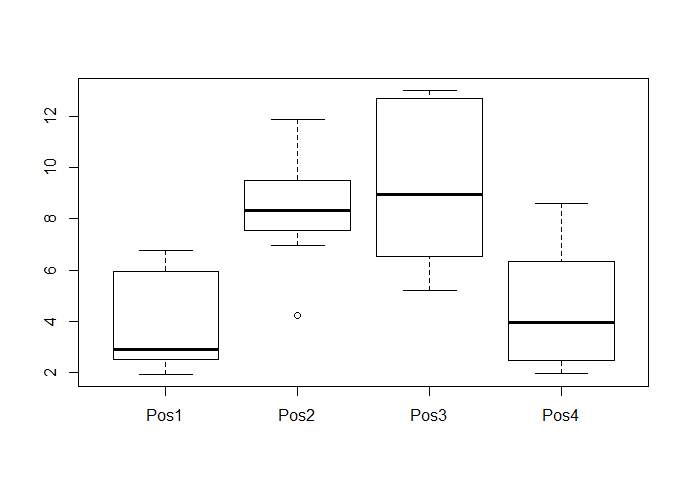
\includegraphics[width = 0.7\textwidth]{Figure/Rplot.png} 
\caption{Boksplot over hvor indbydende hver af de fire hovedpositioner perciperes.}
\label{fig:boksplot}
\end{figure}
\noindent
%
Data analyseres med en \textit{One-way Repeated Measures ANOVA}. Hvor \textit{one-way} refererer til antallet af uafhængige variable, som i dette tilfælde er én; robottens hovedposition. \textit{Repeated measures} refererer til, at samtlige testpersoner præsenteres for samtlige stimuli. Da formålet med denne test er at undersøge hvor indbydende en robot perciperes afhængigt af dens hovedposition, er den afhængige variabel testpersonernes individuelle respons angivet på skalaen. Den indsamlede data er af typen interval data, hvilket skyldes at VAS er en kontinuerlig skala. 

Ydermere dækker den uafhængige variabel over fire kategorier; de fire forskellige hovedpositioner, er det ligeledes oplagt at anvende en ANOVA, da det ønskes at sammenligne mere end to kategorier.\blankline
%
Følgende antagelser skal overholdes for at udføre en \textit{One-way Repeated Measures ANOVA}, \parencite[ss. 507-509]{PDF:ExploringAssumptions}: \blankline  
%
\begin{itemize}
	\item \textbf{Den afhængige variabel skal som minimum være målt på interval skala.}\\
	Vurderingen givet på skalaen er målt på en interval skala og opfylder dermed denne antagelse.
	\item \textbf{Der skal være homogen varians. }\\
	For at teste om der er homogen varians udføres \textit{Levene's test}. Testresultatet er $F(3.28)=1.09, p=0.37$, hvorfor der ikke er signifikant forskel og dermed er antagelsen om homogen varians opfyldt. 
	\item \textbf{Data skal være normalfordelt.}\\
	For teste om der er normalfordeling udføres en \textit{Shapiro-Wilk test}. Testresultatet er $W=0.94, p=0.09$, hvorfor der ikke er signifikant forskel og dermed er antagelsen om normalfordeling er opfyldt.
	\item \textbf{Uafhængig data.}\\
	Testpersonernes respons er uafhængige; testperson 1 har ikke indflydelse på de resterende testpersoners respons. Dog er der afhængighed mellem de fire konditioner testpersonerne præsenteres for.\blankline
\end{itemize}
\noindent
%
Da alle antagelser for at udføre en \textit{One-way Repeated Measures ANOVA} er opfyldt, udføres denne i \textit{rStudio}. Testresultatet er $F(3.21)=13.7, p=4.4*e^{-4}$, hvilket indikerer at der er signifikant effekt af robottens hovedposition på hvor indbydende robotten perciperes.

Baseret på dette resultat er det kun muligt at konkludere, at der er signifikant forskel mellem hvordan hovedpositionerne perciperes i forhold til hvor indbydende robotten er, det er derfor ikke muligt at afgøre hvor den signifikante forskel er. For at undersøge hvor forskellen er udføres der en \textit{Post Hoc test} af typen \textit{Pairwise Comparison}, hvilket udføres med t-tests, \parencite[s. 1171]{PDF:PairwiseComparison}. Testresultatet fremgår af \autoref{fig:sammenligning}.
%
\begin{figure}[H]
\centering
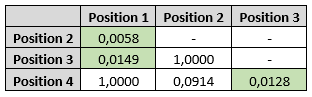
\includegraphics[width = 0.5\textwidth]{Figure/PostHocExcel.PNG} 
\caption{Sammenligning mellem vurderingerne af hvor indbydende robotten perciperes i henhold til dens hovedposition. Grøn markering angiver signifikante forskelle.}
\label{fig:sammenligning}
\end{figure}
\noindent
%
Baseret på \autoref{fig:sammenligning} fremgår det at både position 2 og position 3 er signifikant forskellige fra position 1. Sammenholdes dette med \autoref{fig:boksplot} kan det konkluderes at både position 2 og position 3 perciperes som værende mere indbydende end position 1. I tillæg er der signifikant forskel mellem position 3 og position 4, hvor position 3 perciperes som værende mere indbydende. Det er dog bemærkelsesværdigt at det ikke er tilfældet mellem position 2 og position 4, hvor der ikke fremgår en signifikant forskel, jævnfør \autoref{fig:sammenligning}.
%

